%%%%%%%%%%%%%%%%%%%%%%%%%%%%%%%%%%%%%%%%%
% Beamer Presentation
% LaTeX Template
% Version 1.0 (10/11/12)
%
% This template has been downloaded from:
% http://www.LaTeXTemplates.com
%
% License:
% CC BY-NC-SA 3.0 (http://creativecommons.org/licenses/by-nc-sa/3.0/)
%
%%%%%%%%%%%%%%%%%%%%%%%%%%%%%%%%%%%%%%%%%

%----------------------------------------------------------------------------------------
%	PACKAGES AND THEMES
%----------------------------------------------------------------------------------------

\documentclass{beamer}

\mode<presentation> {

% The Beamer class comes with a number of default slide themes
% which change the colors and layouts of slides. Below this is a list
% of all the themes, uncomment each in turn to see what they look like.

%\usetheme{default}
%\usetheme{AnnArbor}
%\usetheme{Antibes}
%\usetheme{Bergen}
%\usetheme{Berkeley}
%\usetheme{Berlin}
%\usetheme{Boadilla}
%\usetheme{CambridgeUS}
%\usetheme{Copenhagen}
%\usetheme{Darmstadt}
%\usetheme{Dresden}
%\usetheme{Frankfurt}
%\usetheme{Goettingen}
%\usetheme{Hannover}
%\usetheme{Ilmenau}
%\usetheme{JuanLesPins}
%\usetheme{Luebeck}
\usetheme{Madrid}
%\usetheme{Malmoe}
%\usetheme{Marburg}
%\usetheme{Montpellier}
%\usetheme{PaloAlto}
%\usetheme{Pittsburgh}
%\usetheme{Rochester}
%\usetheme{Singapore}
%\usetheme{Szeged}
%\usetheme{Warsaw}

% As well as themes, the Beamer class has a number of color themes
% for any slide theme. Uncomment each of these in turn to see how it
% changes the colors of your current slide theme.

%\usecolortheme{albatross}
%\usecolortheme{beaver}
%\usecolortheme{beetle}
%\usecolortheme{crane}
%\usecolortheme{dolphin}
%\usecolortheme{dove}
%\usecolortheme{fly}
%\usecolortheme{lily}
%\usecolortheme{orchid}
%\usecolortheme{rose}
%\usecolortheme{seagull}
%\usecolortheme{seahorse}
%\usecolortheme{whale}
%\usecolortheme{wolverine}

%\setbeamertemplate{footline} % To remove the footer line in all slides uncomment this line
%\setbeamertemplate{footline}[page number] % To replace the footer line in all slides with a simple slide count uncomment this line

%\setbeamertemplate{navigation symbols}{} % To remove the navigation symbols from the bottom of all slides uncomment this line
}
\usepackage[english]{babel}
\usepackage{authblk}
\usepackage{amsthm, calc}
\usepackage{amsfonts}
\usepackage{graphicx}
\graphicspath{ {./images/} }



% Set page size and margins
% Replace `letterpaper' with `a4paper' for UK/EU standard size
% Useful packages
\usepackage{amsmath}
\usepackage{graphicx}
\usepackage{graphicx} % Allows including images
\usepackage{booktabs} % Allows the use of \toprule, \midrule and \bottomrule in tables

%----------------------------------------------------------------------------------------
%	TITLE PAGE
%----------------------------------------------------------------------------------------

\title[Math Report]{Analysis of the Stability in Nonlinear Ordinary Differential
Equations} % The short title appears at the bottom of every slide, the full title is only on the title page

\author{Ranitha Mataraarachchi} % Your name
\institute[UoP] % Your institution as it will appear on the bottom of every slide, may be shorthand to save space
{
Department of Engineering Mathematics, University of Peradeniya, Sri Lanka \\ % Your institution for the title page
\medskip
\textit{Ranitha Mataraarachchi} % Your email address
}
\date{\today} % Date, can be changed to a custom date

\begin{document}

\begin{frame}
\titlepage % Print the title page as the first slide
\end{frame}

\begin{frame}
\frametitle{Overview} % Table of contents slide, comment this block out to remove it
\tableofcontents % Throughout your presentation, if you choose to use \section{} and \subsection{} commands, these will automatically be printed on this slide as an overview of your presentation
\end{frame}

%----------------------------------------------------------------------------------------
%	PRESENTATION SLIDES
%----------------------------------------------------------------------------------------

%------------------------------------------------
\section{Nonlinear Systems} 
\subsection{Ordinary Differential Equations} 
\begin{frame}{Ordinary Differential Equations}
    Differential equations, which involve functions and their derivatives, are widely applied in physics, engineering, and biology. Mathematicians are interested in finding and characterizing the solutions (equilibrium points) to these equations. 
    \newline
    \newline
    A system of $n^{th}$ order Autonomous Ordinary Differential Equation (ODE) can be represented as:
    \begin{equation}\label{auto}
        \dot{X} = F(X)
    \end{equation}
    for some vector valued function $F$. Here we assume $F$ is a collection of continuous differentiable functions.
\end{frame}



\subsection{Equilibrium points of an Ordinary Differential Equation}

\begin{frame}{Equilibrium points of an Ordinary Differential Equation}
    It is clear that for a system to achieve equilibrium the rate of change $\dot{X}$ must be $0$.
\begin{definition}
    An equilibrium of the n dimensional system $\dot{X} = F(X)$ is a vector $X^* \in \mathbb{R}^n$  such that $F(X^*)=0.$
\end{definition}
\end{frame}


\section{Definition of Stability}
\begin{frame}{Stable, unstable and asymptotically stable systems}
Any equilibrium point can be shifted to the origin through a variable transformation.
    \begin{definition}
    The equilibrium point $X=0$ of $\dot{X}=F(X)$ is
    \begin{itemize}
        \item \textbf{stable} if, for each $\epsilon > 0$, there is $\delta = \delta(\epsilon)>0$ such that
        $$\|X(0)\|<\delta \implies \|X(t)\|<\epsilon, \forall t\geq 0.$$

        \item \textbf{unstable} if it is not stable.

        \item \textbf{asymptotically stable} if it is stable \emph{and} $\delta$ can be chosen such that
        $$\|X(0)\|<\delta \implies \lim_{t \to \infty} X(t)=0.$$
    \end{itemize}
\end{definition}
Here, $\|\|$ represents the $L_2$ norm.
\end{frame}

\section{Stability Analysis Using Linearization}
\begin{frame}{Stability of nonlinear systems by linearization}
    We can check the stability of nonlinear systems by linearizing the system in the vicinity of equilibrium points. After that, we can use a similar theorem as before to arrive at conclusions regarding the nonlinear system. 
    \newline\newline
    Recall that the Jacobian matrix of $F$ evaluated at $X=0$ can be represented as, 
    \[
A = \begin{bmatrix}
    \frac{\partial{f_1}}{\partial{x_1}}(0) & \frac{\partial{f_1}}{\partial{x_2}}(0) & \hdots & \frac{\partial{f_1}}{\partial{x_n}}(0) \\
    \frac{\partial{f_2}}{\partial{x_1}}(0) & \frac{\partial{f_2}}{\partial{x_2}}(0) & \hdots & \frac{\partial{f_2}}{\partial{x_n}}(0) \\
    \vdots & \vdots & \ddots & \vdots \\
    \frac{\partial{f_n}}{\partial{x_1}}(0) & \frac{\partial{f_n}}{\partial{x_2}}(0) & \hdots & \frac{\partial{f_n}}{\partial{x_n}}(0) \\
\end{bmatrix}.
\]
\end{frame}
\begin{frame}{Stability of nonlinear systems by linearization}
    \begin{theorem}\label{t2}
    Let $X=0$ be an equilibrium point for the nonlinear system
    $$\dot{X}=F(X)$$
    where all the functions $f_1,f_2,\dots,f_n$ in $F$ are continuously differentiable in the neighbourhood of the origin. Let $A$ be the Jacobian matrix of $F$ evaluated at $X=0.$
    Then, 
    \begin{itemize}
        \item The origin is asymptotically stable if all eigenvalues $\lambda_i$ of $A$ satisfy $Re(\lambda_i)<0.$
        \item The origin is unstable if $Re(\lambda_i)>0$ for one or more eigenvalues of $A.$
    \end{itemize}
\end{theorem}
\end{frame}


\section{Lyapunov’s Stability Theorem}
\begin{frame}{Lyapunov’s Stability Theorem}
    \begin{itemize}
        \item We can deduce the stability of the system by observing what happens to the energy of the system over time.
        \item If the energy of the system remains constant or reduces over time, then the system is stable.
        \item If the energy increases over time then the system is not stable. 
        \item By utilizing the concept of energy, Lyapunov’s Stability Theorem can be formulated to deduce the stability of a system.
    \end{itemize}
     
    \begin{figure}[h]
    \centering
    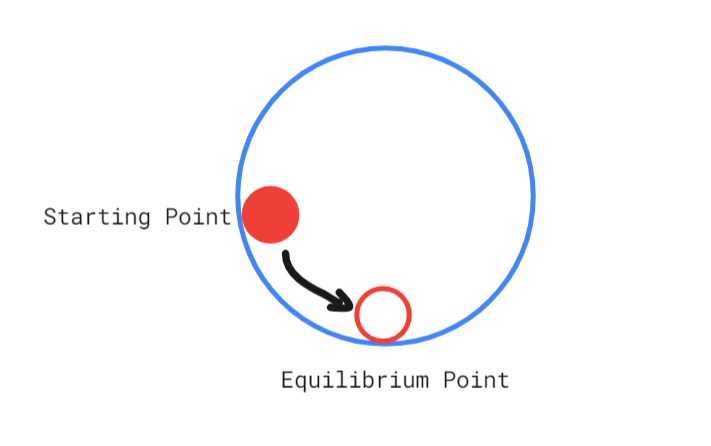
\includegraphics[scale=0.5]{images/ball.png}
    \end{figure}
    
\end{frame}

\begin{frame}{Lyapunov’s Stability Theorem} 

    \begin{theorem}\label{t3}
    Let $X=0$ be an equilibrium point for the system $\dot{X}=F(X)$ and $D \subset \mathbb{R}^n$ be a domain containing $X=0.$ Let $V:D\to \mathbb{R}$ be a continuously differentiable function such that 
    $$V(0)=0 \text{  and  } V(X)>0 \text{  for  } X\in D\setminus \{0\}.$$
    If 
    $$\frac{dV(X)}{dt}\leq 0 \text{  for  } X\in D,$$
    then $X=0$ is stable. Moreover, if
    $$\frac{dV(X)}{dt} < 0 \text{  for  } X\in  D\setminus \{0\}$$
    then $X=0$ is asymptotically stable.
\end{theorem}
Here $V(X)$ is called the \emph{Lyapunov's function}.
\end{frame}

\section{Lotka-Volterra Predator vs. Prey Model}
\begin{frame}{Lotka-Volterra Predator vs. Prey Model}
    The Lotka–Volterra model describes the dynamics of interacting predator and prey species with a set of two nonlinear differential equations.

    \begin{align*}
  \dot{x_1} &= ax_1-bx_1x_2\\
  \dot{x_2} &= -cx_2 + dx_1x_2.
\end{align*}

\begin{itemize}
    \item $x_1,x_2$ are the population densities of pray and predators respectively.
    \item $\dot{x_1},\dot{x_2}$ are the instantaneous growth rates of the two populations and $t$ represents time.
    \item $a$ and $b$ represent, respectively, the highest per capita growth rate of prey and the impact of predator presence on the rate of prey growth.
    \item $c$ and $d$, respectively, characterize the per capita death rate of predators and the influence of prey presence on the predator's growth rate.
    \item All parameters $a,b,c,d$ are positive and real.
\end{itemize}

\end{frame}

\begin{frame}{Equilibrium points}
    We can represent this system as
\begin{equation}\label{lotka}
    \dot{X}=F(X).
\end{equation}

This system has two equilibrium points: 

\begin{itemize}
    \item $(0,0)$ (trivial equilibrium point) 
    \item $(\frac{c}{d},\frac{a}{b})$ (nontrivial equilibrium point)
\end{itemize}
\end{frame}

\begin{frame}{Trivial equilibrium point}
    We can linearize the system in a neighbourhood of the equilibrium point to analyse the stability. We will find the eigenvalues of the Jacobian of $F$ at $X=0.$

    \[
A =  \begin{bmatrix}
    a & 0 \\
    0 & -c
\end{bmatrix}.
\]
Eigenvalues are $\lambda_1=a$ and $\lambda_2=-c.$ Since we get a positive eigenvalue, the system is \textbf{unstable} at the trivial equilibrium point. 
\end{frame}

\begin{frame}{Trivial equilibrium point numerical simulation}
    \begin{figure}[h]
\centering
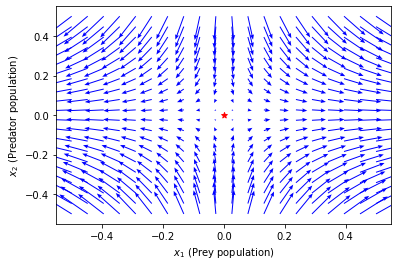
\includegraphics[scale=0.60]{images/origin.png}
\caption{Flow lines near the equilibrium point at the origin.}
\end{figure}
\end{frame}

\begin{frame}{Nontrivial equilibrium point}
Stability analysis by linearization is not conclusive at this point since the eigenvalues of the Jacobian matrix becomes purely imaginary ($Re(\lambda)=0$).
\newline\newline
Therefore, we resolve to conduct stability analysis using the Lyapunov's method.
Consider the function 
\begin{equation}\label{energy}
    V(y_1,y_2) = dy_1 - c \ln\left(\frac{dy_1+c}{d}\right)+by_2- a \ln\left(\frac{by_2+a}{b}\right)+K,
\end{equation}

where $a,b,c,d$ are the Lotka-Volterra parameters and $K$ is a constant. Then, by differentiating we see that
$$\frac{V(Y)}{dt}=0.$$ Thus, by Lyapunov's theorem we can conclude that the above system is \textbf{stable} at the equilibrium point $Y=(0,0)$.
\end{frame}

\begin{frame}{Nontrivial equilibrium point numerical simulation}
    \begin{figure}[h]
\centering
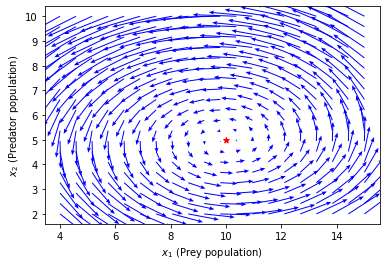
\includegraphics[scale=0.60]{images/nontrivial.png}
\caption{Flow lines near the nontrivial equilibrium point.}
\end{figure}
\end{frame}

\begin{frame}{References}
\nocite{*}
\bibliographystyle{plain}
\bibliography{sample}
\end{frame}

%------------------------------------------------

\begin{frame}
\Huge{\centerline{Thank You}}
\end{frame}

%----------------------------------------------------------------------------------------

\end{document}